\documentclass[10pt,a4paper]{article}

% =========================================================================
% Packages
% =========================================================================
\usepackage[utf8]{inputenc}
\usepackage[T1]{fontenc}
\usepackage{lmodern}
\usepackage{geometry}
\usepackage{graphicx}
\graphicspath{{Gambar/}}
\usepackage{amsmath,amssymb}
\usepackage{fancyhdr}
\usepackage{titlesec}
\usepackage{booktabs}
\usepackage{tabularx}
\usepackage{array}
\usepackage{caption}
\usepackage{subcaption}
\usepackage{algorithm}
\usepackage{algpseudocode}
\usepackage{hyperref}
\usepackage{microtype}
\usepackage{url}
\usepackage{cite}

% =========================================================================
% Page Geometry & Margins (EPROTIK Standard: A4 Paper, Margins: 2.5 cm all sides)
% =========================================================================
\geometry{
  a4paper,
  top=2.5cm,
  bottom=2.5cm,
  left=2.5cm,
  right=2.5cm,
  headheight=45pt,
  headsep=12pt,
  footskip=22pt
}

% Paragraph settings: Justified, single space, compact spacing for <= 10 pages
\setlength{\parindent}{0pt}
\setlength{\parskip}{4pt}
\linespread{1.0}

% Float Spacing Adjustments
\setlength{\floatsep}{8pt plus 2pt minus 2pt}
\setlength{\textfloatsep}{10pt plus 2pt minus 2pt}
\setlength{\intextsep}{8pt plus 2pt minus 2pt}

% Hyperlink configuration
\hypersetup{
  colorlinks=true,
  linkcolor=blue,
  citecolor=blue,
  urlcolor=blue
}

% =========================================================================
% Header & Footer Settings
% =========================================================================
\pagestyle{fancy}
\fancyhf{}
\fancyhead[L]{\fontsize{9pt}{11pt}\selectfont eProceeding of TIK}
\fancyfoot[R]{\fontsize{9pt}{11pt}\selectfont\thepage}
\renewcommand{\headrulewidth}{0.4pt}
\renewcommand{\footrulewidth}{0pt}

% First page header
\fancypagestyle{firstpage}{
  \fancyhf{}
  \fancyhead[L]{%
    \begin{minipage}[c]{0.78\textwidth}
      {\fontsize{10pt}{12pt}\selectfont\textbf{eProceeding of TIK}}\\[2pt]
      {\fontsize{8.5pt}{10.5pt}\selectfont E-ISSN: 2797-1724, P-ISSN: 3031-1454}\\[1pt]
      {\fontsize{8.5pt}{10.5pt}\selectfont Vol. 7 No. 1 2027 pp. 1--10}
    \end{minipage}%
  }
  \fancyhead[R]{%
    \begin{minipage}[c]{0.20\textwidth}
      \raggedleft
      \IfFileExists{Gambar/elvira_image5.png}{
\includegraphics[height=1.05cm]{elvira_image5.png}}{%
        \IfFileExists{Gambar/image1.png}{
\includegraphics[height=1.05cm]{image1.png}}{}%
      }
    \end{minipage}%
  }
  \fancyfoot[R]{\fontsize{9pt}{11pt}\selectfont\thepage}
  \renewcommand{\headrulewidth}{0.5pt}
  \renewcommand{\footrulewidth}{0pt}
}

% =========================================================================
% Section Headings Formatting
% Level 1: 13pt Bold
% Level 2: 11pt Bold
% Level 3: 10pt Bold
% =========================================================================
\titleformat{\section}
  {\fontsize{13pt}{16pt}\bfseries}{\thesection.}{0.5em}{}
\titlespacing*{\section}{0pt}{10pt}{3pt}

\titleformat{\subsection}
  {\fontsize{11pt}{14pt}\bfseries}{\thesubsection}{0.5em}{}
\titlespacing*{\subsection}{0pt}{7pt}{2pt}

\titleformat{\subsubsection}
  {\fontsize{10pt}{12pt}\bfseries}{\thesubsubsection}{0.5em}{}
\titlespacing*{\subsubsection}{0pt}{5pt}{2pt}

% Caption styles
\captionsetup{font={small},labelfont=bf,justification=centering}
\captionsetup[table]{position=top,skip=3pt}
\captionsetup[figure]{position=bottom,skip=4pt}

% =========================================================================
% Document Body
% =========================================================================
\begin{document}
\thispagestyle{firstpage}

% --- Article Title (19pt Bold) ---
{\fontsize{19pt}{23pt}\bfseries\raggedright Perbandingan Akurasi ChatGPT Menggunakan Chain-of-Thought dan Non-Chain-of-Thought pada IndoMMLU\par}
\vspace{6pt}

% --- Authors (10pt Regular) ---
{\fontsize{10pt}{12pt}\selectfont Elvira Gladys Samsul$^{1}$, Muhammad Arhami$^{2*}$, Muhammad Rizka$^{3}$\par}
\vspace{3pt}

% --- Affiliations (8.5pt) ---
{\fontsize{8.5pt}{11pt}\selectfont
$^{1,2,3}$ Jurusan Teknologi Informasi dan Komputer, Politeknik Negeri Lhokseumawe, Jl. Banda Aceh--Medan Km. 280,3 Buketrata, Lhokseumawe 24301, Indonesia\par}
\vspace{3pt}

% --- Corresponding Author (8.5pt) ---
{\fontsize{8.5pt}{11pt}\selectfont
*Penulis Korespondensi: \href{mailto:mhselvira@gmail.com}{mhselvira@gmail.com}\par}
\vspace{3pt}

% --- Open Access License (8pt) ---
{\fontsize{8pt}{10pt}\selectfont
This is an open access article under the \href{https://creativecommons.org/licenses/by-sa/4.0/}{CC BY-SA} license. 
\IfFileExists{Gambar/elvira_image1.png}{\raisebox{-0.10cm}{
\includegraphics[height=0.40cm]{elvira_image1.png}}}{}\par}

\vspace{4pt}
\noindent\rule{\textwidth}{0.4pt}
\vspace{2pt}

% --- Abstrak Indonesia (9.5pt Bold-Italic Content) ---
{\fontsize{13pt}{15pt}\bfseries Abstrak\par}
\vspace{3pt}

{\fontsize{9.5pt}{12pt}\bfseries\itshape
Perkembangan Large Language Model (LLM) seperti ChatGPT meningkatkan kemampuan pemahaman bahasa alami, namun kemampuannya dalam konteks bahasa dan budaya lokal Indonesia masih perlu dievaluasi karena sebagian besar pengujian dilakukan menggunakan dataset berbahasa Inggris. Penelitian ini mengukur akurasi jawaban GPT-4o mini pada soal Multiple Choice Question (MCQ) dataset IndoMMLU domain bahasa menggunakan algoritma Levenshtein Distance, serta membandingkan efektivitas metode Chain-of-Thought (CoT) dan Non-Chain-of-Thought (Non-CoT). Pengujian dilakukan melalui empat skenario terhadap sembilan domain bahasa daerah dengan total hingga 900 soal, mengukur nilai similarity, akurasi exact match, penggunaan token, dan waktu respons. Hasil menunjukkan pengujian per domain menghasilkan similarity rata-rata 65,42\% (CoT) dan 63,81\% (Non-CoT), dengan 483 dan 454 jawaban benar dari 900 soal. Pada pengujian gabungan skala besar, Non-CoT justru lebih stabil dengan similarity tertinggi 70,18\% dibanding CoT 69,37\%. Bahasa Indonesia mencapai similarity tertinggi (95,92\%), sedangkan bahasa daerah lain berkisar 55,49\%--77,23\%. CoT membutuhkan token sekitar 5,2 kali lebih besar dan waktu respons empat hingga enam kali lebih lama dibanding Non-CoT. Temuan ini menunjukkan bahwa efektivitas Chain-of-Thought tidak konsisten meningkatkan kualitas jawaban GPT-4o mini, melainkan bergantung pada karakteristik domain bahasa dan skala pengujian.\par}

\vspace{4pt}
{\fontsize{9.5pt}{12pt}\bfseries\itshape Kata Kunci: \normalfont\itshape Chain-of-Thought, ChatGPT, IndoMMLU, Levenshtein Distance, Multiple Choice Question.\par}

\vspace{4pt}
% --- Abstract English ---
{\fontsize{9.5pt}{12pt}\bfseries\itshape
\noindent\textbf{Abstract} --- The emergence of Large Language Models (LLMs) such as ChatGPT has significantly enhanced natural language understanding; however, their reasoning capabilities on Indonesian local languages and cultural nuances require rigorous evaluation since global benchmarks predominantly focus on English. This study assesses the accuracy of GPT-4o mini on Multiple Choice Questions (MCQ) from the IndoMMLU benchmark across local language domains using the Levenshtein Distance algorithm, comparing the efficacy of Chain-of-Thought (CoT) against Non-Chain-of-Thought (Non-CoT) prompting. Experiments were conducted across four evaluation scenarios covering nine regional language domains with up to 900 test items, tracking similarity scores, exact-match accuracy, token consumption, and response latency. In single-domain evaluations, CoT achieved an average similarity of 65.42\% compared to 63.81\% for Non-CoT (483 vs. 454 correct answers out of 900). Conversely, in large-scale multi-domain evaluations, Non-CoT proved more stable, attaining a peak similarity of 70.18\% versus 69.37\% for CoT. Indonesian achieved the highest similarity (95.92\%), whereas local languages ranged between 55.49\% and 77.23\%. Furthermore, CoT consumed approximately 5.2 times more tokens and quadrupled response latency compared to Non-CoT. These empirical findings indicate that Chain-of-Thought does not uniformly improve GPT-4o mini's performance in low-resource regional languages, exhibiting strong dependency on linguistic domain characteristics and testing scale.\par}

\vspace{4pt}
{\fontsize{9.5pt}{12pt}\bfseries\itshape Keywords: \normalfont\itshape Chain-of-Thought, ChatGPT, IndoMMLU, Levenshtein Distance, Multiple Choice Question.\par}

\vspace{3pt}
\noindent\rule{\textwidth}{0.4pt}
\vspace{4pt}

% =========================================================================
% Section 1: Introduction
% =========================================================================
\section{PENDAHULUAN}

\textit{Large Language Model} (LLM) menunjukkan kemajuan yang sangat signifikan dalam bidang pemrosesan bahasa alami (\textit{Natural Language Processing}), terutama dalam pemahaman konteks, penalaran multi-langkah, dan penyelesaian tugas akademik berbasis teks maupun \textit{Multiple Choice Question} (MCQ) \cite{kocmi2022findings, takumu2023indommlu}. Model LLM generasi mutakhir seperti ChatGPT berbasis GPT-4 dan GPT-4o mini telah menunjukkan performa superior pada berbagai tolok ukur (\textit{benchmark}) internasional, bahkan pada sebagian domain penalaran formal dilaporkan mampu menyamai atau melampaui kemampuan rata-rata manusia \cite{takumu2023indommlu, li2024can, brown2020language}.

Namun demikian, capaian performa tinggi tersebut sebagian besar dievaluasi menggunakan dataset berbahasa Inggris dan domain pengetahuan global, sehingga belum sepenuhnya merepresentasikan kemampuan model dalam memahami bahasa daerah serta konteks budaya lokal Indonesia \cite{takumu2023indommlu}. Keterbatasan ini mendorong dikembangkannya IndoMMLU sebagai \textit{benchmark} komprehensif pertama di Indonesia untuk menguji kemampuan LLM pada berbagai tingkatan domain keilmuan dan rumpun bahasa daerah \cite{kocmi2022findings}. Evaluasi awal pada IndoMMLU menunjukkan bahwa performa model bahasa pada bahasa non-Inggris dan bahasa berdaya komputasi rendah (\textit{low-resource languages}) masih mengalami penurunan akurasi yang tajam dibandingkan bahasa utama \cite{xu2024reasoning, teh2024impact}.

Permasalahan evaluasi LLM pada domain bahasa Indonesia tidak hanya bersumber dari keterbatasan korpus pelatihan, tetapi juga sangat dipengaruhi oleh strategi perancangan instruksi (\textit{prompting strategy}) yang diterapkan. Sebagian besar evaluasi MCQ pada literatur sebelumnya hanya mencocokkan huruf opsi jawaban (misalnya: A, B, C, atau D) terhadap kunci referensi \cite{kocmi2022findings, li2024can, xu2024reasoning}, tanpa mengevaluasi kesesuaian narasi penjelasan atau teks jawaban akhir yang diproduksi model. Metode \textit{Chain-of-Thought} (CoT) \textit{prompting} diajukan sebagai paradigma baru yang mengarahkan model untuk menghasilkan langkah-langkah penalaran terstruktur (\textit{intermediate reasoning steps}) sebelum menentukan kesimpulan akhir \cite{wei2023chain, kojima2023large, jia2025comprehensive}. Meskipun CoT terbukti efektif pada tugas aritmatika dan logika simbolik, efektivitasnya pada bahasa daerah yang memiliki struktur sintaksis unik dan data leksikal terbatas masih menyisakan perdebatan akademis \cite{kim2023cot, ji2024chain}.

Selain itu, metode evaluasi kesesuaian teks berbasis pencocokan eksak (\textit{Exact Match}) bersifat terlalu kaku karena menganggap jawaban salah total meskipun terdapat variasi ejaan minor atau sinonim. Algoritma Levenshtein Distance menawarkan pendekatan kuantitatif yang objektif dan granular dengan mengukur jumlah operasi penyuntingan minimum (penyisipan, penghapusan, dan substitusi) yang dibutuhkan untuk mengubah teks respons model menjadi teks referensi \cite{lind2023comparing, song2024sidildng, berger2021levenshtein, sandamette2025}.

Penelitian ini bertujuan untuk mengukur dan membandingkan akurasi jawaban ChatGPT model GPT-4o mini pada soal MCQ dataset IndoMMLU domain bahasa daerah menggunakan metode \textit{Chain-of-Thought} dan \textit{Non-Chain-of-Thought} berbasis algoritma Levenshtein Distance. Evaluasi dilakukan secara sistematis melalui empat skenario pengujian terhadap 9 domain bahasa (Bahasa Indonesia, Jawa, Sunda, Minangkabau/Lampung, Bali, Makassar, Madura, Dayak Ngaju, dan Banjar) dengan total 900 butir soal. Selain mengukur akurasi kesesuaian narasi (\textit{similarity score}) dan \textit{exact match}, penelitian ini menganalisis secara mendalam \textit{trade-off} efisiensi komputasi yang mencakup konsumsi token dan waktu respons (\textit{latency}).

% =========================================================================
% Section 2: Methods
% =========================================================================
\section{METODE PENELITIAN}

\subsection{Alur Penelitian dan Arsitektur Sistem EvalGPT}
Penelitian ini dilaksanakan menggunakan pendekatan eksperimen kuantitatif dengan mengembangkan sistem otomasi evaluasi berbasis web bernama \textbf{EvalGPT}. Alur penerapan metode \textit{Chain-of-Thought} dan pengukuran akurasi Levenshtein Distance diilustrasikan pada Gambar \ref{fig:flow_cot_lev}.

\begin{figure}[htbp]
  \centering
  \begin{subfigure}[b]{0.48\textwidth}
    \centering
    \IfFileExists{Gambar/skripsi_elvira_image33.png}{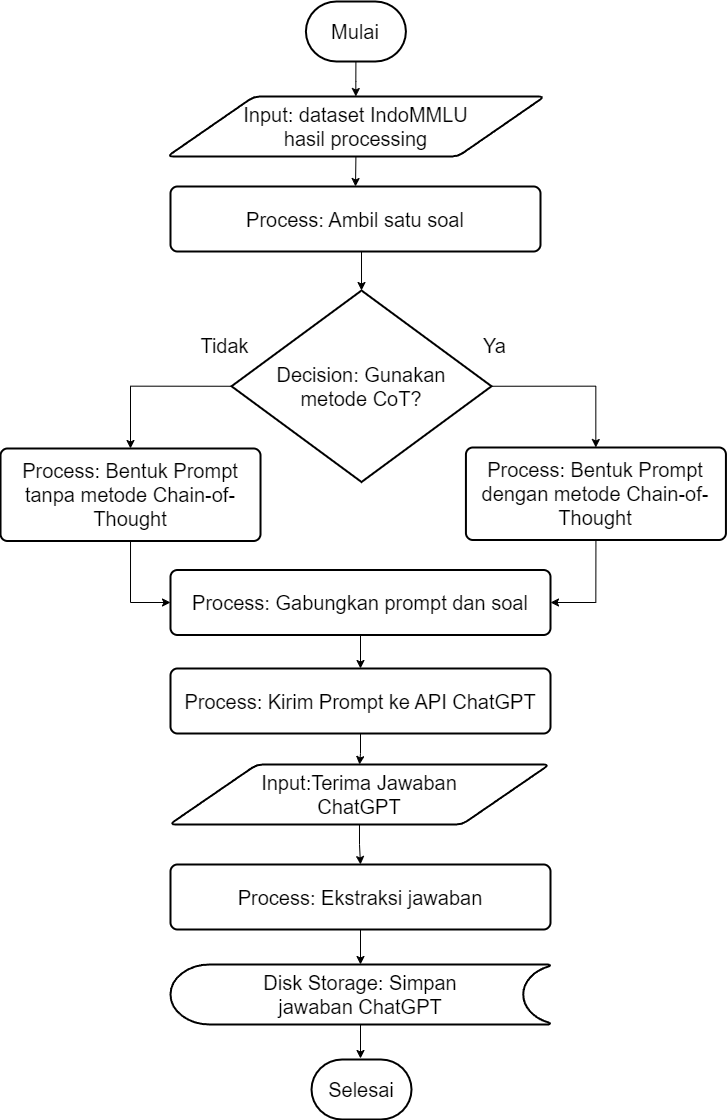
\includegraphics[width=\textwidth]{skripsi_elvira_image33.png}}{\fbox{Flowchart CoT}}
    \caption{Alur Penerapan Metode Chain-of-Thought}
    \label{fig:flow_cot}
  \end{subfigure}
  \hfill
  \begin{subfigure}[b]{0.48\textwidth}
    \centering
    \IfFileExists{Gambar/skripsi_elvira_image34.png}{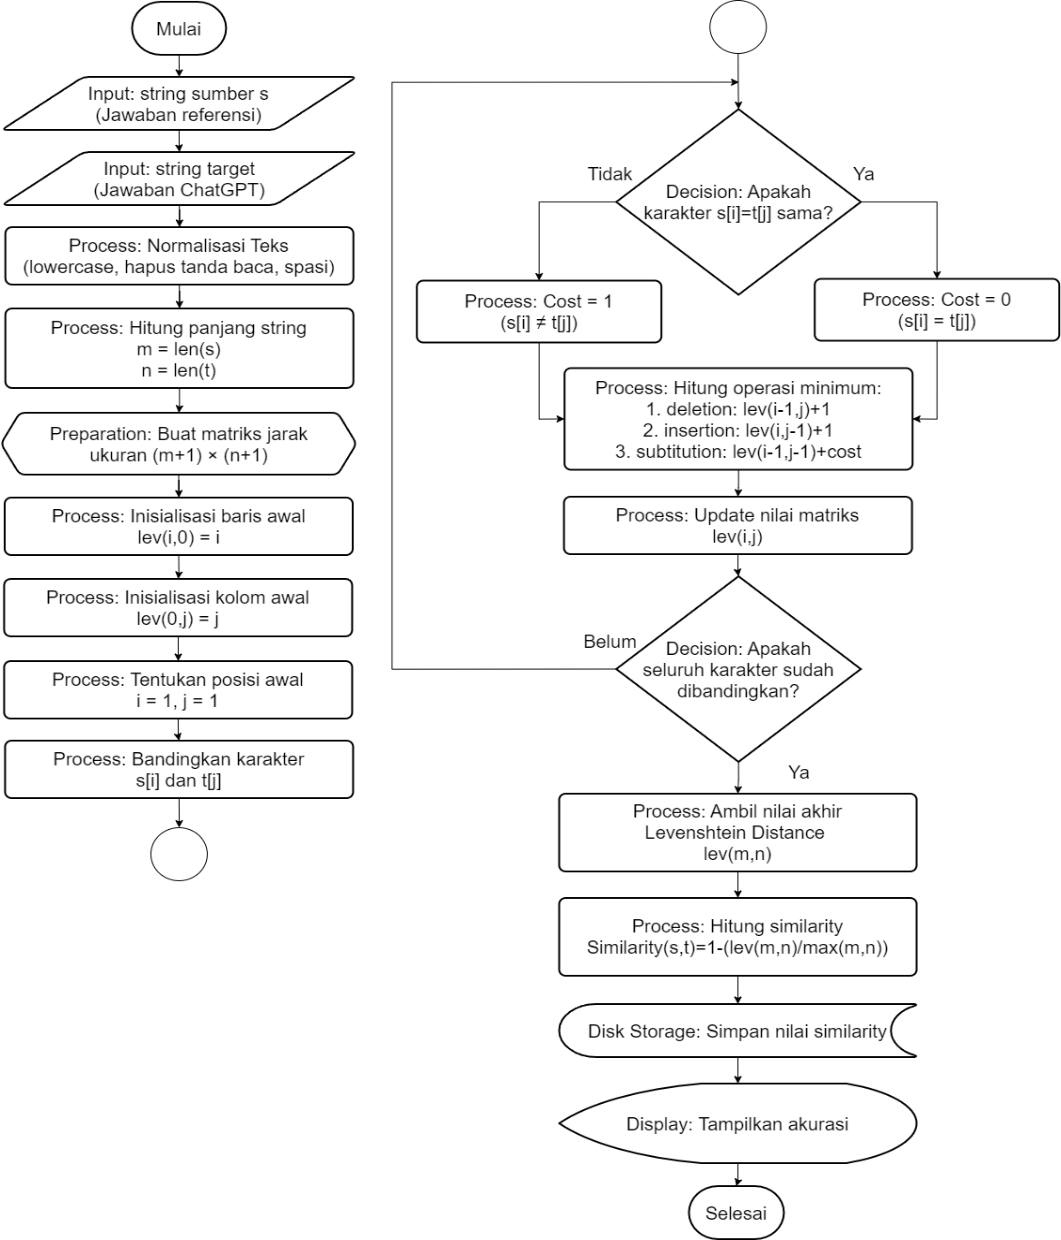
\includegraphics[width=\textwidth]{skripsi_elvira_image34.png}}{\fbox{Flowchart Levenshtein}}
    \caption{Alur Perhitungan Levenshtein Distance}
    \label{fig:flow_lev}
  \end{subfigure}
  \caption{Diagram Alur Metode Penelitian: (a) Mekanisme Inferensi CoT, (b) Komputasi Levenshtein Distance}
  \label{fig:flow_cot_lev}
\end{figure}

\subsection{Dataset IndoMMLU Domain Bahasa}
Dataset yang digunakan bersumber dari tolok ukur resmi IndoMMLU \cite{kocmi2022findings}. Korpus difokuskan pada 9 subjek domain bahasa daerah di Indonesia dengan total 900 soal pilihan ganda (masing-masing 100 butir soal):
\begin{enumerate}
    \item Bahasa Indonesia (100 soal)
    \item Bahasa Jawa (100 soal)
    \item Bahasa Sunda (100 soal)
    \item Bahasa Lampung (100 soal)
    \item Bahasa Bali (100 soal)
    \item Bahasa Makassar (100 soal)
    \item Bahasa Banjar (100 soal)
    \item Bahasa Madura (100 soal)
    \item Bahasa Dayak Ngaju (100 soal)
\end{enumerate}

Setiap butir data memuat atribut pertanyaan (\textit{question}), opsi pilihan jawaban (A, B, C, D), dan kunci jawaban referensi (\textit{ground truth answer key}).

\subsection{Perancangan Prompt CoT dan Non-CoT}
Untuk membandingkan performa model GPT-4o mini, dirancang dua struktur instruksi (\textit{prompt template}):
\begin{enumerate}
    \item \textbf{Prompt Non-Chain-of-Thought (Non-CoT):} Menginstruksikan model untuk langsung memberikan jawaban akhir tanpa menyertakan proses penalaran:
    \begin{quote}
    \small \texttt{"Jawablah pertanyaan pilihan ganda berikut dengan memilih satu jawaban yang paling tepat. Format jawaban: [Huruf Opsi]. [Teks Jawaban]"}
    \end{quote}
    \item \textbf{Prompt Chain-of-Thought (CoT):} Menerapkan teknik \textit{zero-shot} CoT dengan menambahkan arahan eksplisit penalaran bertahap \cite{kojima2023large}:
    \begin{quote}
    \small \texttt{"Jawablah pertanyaan pilihan ganda berikut. Mari kita pikirkan langkah demi langkah (step-by-step reasoning) terlebih dahulu sebelum menentukan jawaban. Di baris terakhir, tuliskan jawaban akhir dengan format: Jawaban Akhir: [Huruf Opsi]. [Teks Jawaban]"}
    \end{quote}
\end{enumerate}

\subsection{Algoritma Levenshtein Distance dan Pengukuran Kemiripan}
Algoritma Levenshtein Distance digunakan untuk menghitung jarak penyuntingan minimum antara string teks respons model ($a$) dan string teks kunci referensi ($b$). Secara matematis, matriks jarak $\text{lev}_{a,b}(i, j)$ didefinisikan secara rekursif melalui pemrograman dinamis (\textit{dynamic programming}) \cite{lind2023comparing, berger2021levenshtein}:
\begin{equation}
  \text{lev}_{a,b}(i,j) = 
  \begin{cases} 
    \max(i,j) & \text{jika } \min(i,j) = 0, \\
    \min \begin{cases}
      \text{lev}_{a,b}(i-1, j) + 1 \\
      \text{lev}_{a,b}(i, j-1) + 1 \\
      \text{lev}_{a,b}(i-1, j-1) + \mathbf{1}_{(a_i \neq b_j)}
    \end{cases} & \text{lainnya.}
  \end{cases}
  \label{eq:levenshtein}
\end{equation}
di mana $\mathbf{1}_{(a_i \neq b_j)}$ bernilai 0 jika karakter ke-$i$ pada string $a$ sama dengan karakter ke-$j$ pada string $b$, dan bernilai 1 jika berbeda. Nilai akhir jarak diperoleh pada elemen $\text{lev}(a, b) = \text{lev}_{a,b}(|a|, |b|)$.

Tingkat kemiripan (\textit{Similarity Score}) antara respons model dan teks referensi dihitung dalam skala persentase:
\begin{equation}
  \text{Similarity}(a, b) = \left( 1 - \frac{\text{lev}(a, b)}{\max(|a|, |b|)} \right) \times 100\%
  \label{eq:similarity_lev}
\end{equation}

Suatu jawaban dikategorikan sebagai \textbf{Exact Match} ($100\%$ benar) apabila $\text{Similarity}(a, b) = 100\%$ atau huruf opsi dan narasi jawaban identik sempurna dengan kunci referensi.

\subsection{Skenario Pengujian}
Pengujian performa model GPT-4o mini dibagi ke dalam empat skenario komprehensif:
\begin{itemize}
    \item \textbf{Skenario 1 (Per Domain Tunggal):} Menguji 100 soal pada masing-masing dari 9 domain secara terisolasi (total 900 soal).
    \item \textbf{Skenario 2 (Multi-Domain 25 Soal):} Menggabungkan 25 soal acak dari setiap domain (total 225 soal campuran).
    \item \textbf{Skenario 3 (Multi-Domain 50 Soal):} Menggabungkan 50 soal acak dari setiap domain (total 450 soal campuran).
    \item \textbf{Skenario 4 (Multi-Domain 100 Soal):} Menggabungkan seluruh 100 soal dari setiap domain dalam satu sesi pengujian (total 900 soal campuran).
\end{itemize}

% =========================================================================
% Section 3: Results and Discussion
% =========================================================================
\section{HASIL DAN PEMBAHASAN}

\subsection{Hasil Pengujian Skenario 1 (Per Domain Bahasa)}
Hasil pengujian performa GPT-4o mini untuk masing-masing domain bahasa pada Skenario 1 dirangkum pada Tabel \ref{tab:skenario1}.

\begin{table}[htbp]
  \centering
  \caption{Rekapitulasi Hasil Pengujian Per Domain Bahasa (Skenario 1 -- 900 Soal)}
  \label{tab:skenario1}
  \fontsize{8.5pt}{11pt}\selectfont
  \begin{tabular}{clccccc}
    \toprule
    \textbf{No} & \textbf{Domain Bahasa} & \textbf{Similarity NC} & \textbf{Similarity CoT} & \textbf{Benar NC} & \textbf{Benar CoT} & \textbf{Metode Unggul} \\
    \midrule
    1 & Bahasa Lampung      & 61.60\% & 66.92\% & 46/100 (46\%) & 56/100 (56\%) & CoT (+10) \\
    2 & Bahasa Bali         & 55.49\% & 62.14\% & 38/100 (38\%) & 49/100 (49\%) & CoT (+11) \\
    3 & Bahasa Makassar     & 59.88\% & 59.39\% & 37/100 (37\%) & 37/100 (37\%) & Setara \\
    4 & Bahasa Banjar       & 62.77\% & 61.03\% & 45/100 (45\%) & 45/100 (45\%) & Setara \\
    5 & Bahasa Madura       & 59.36\% & 55.06\% & 40/100 (40\%) & 37/100 (37\%) & Non-CoT (+3) \\
    6 & Bahasa Indonesia    & 93.86\% & 95.92\% & 90/100 (90\%) & 94/100 (94\%) & CoT (+4) \\
    7 & Bahasa Dayak Ngaju  & 61.02\% & 57.88\% & 33/100 (33\%) & 33/100 (33\%) & Setara \\
    8 & Bahasa Sunda        & 69.70\% & 73.39\% & 62/100 (62\%) & 66/100 (66\%) & CoT (+4) \\
    9 & Bahasa Jawa         & 76.18\% & 77.23\% & 63/100 (63\%) & 66/100 (66\%) & CoT (+3) \\
    \midrule
    \multicolumn{2}{l}{\textbf{Rata-rata / Total Benar}} & \textbf{63.81\%} & \textbf{65.42\%} & \textbf{454/900 (50.4\%)} & \textbf{483/900 (53.7\%)} & \textbf{CoT Unggul} \\
    \bottomrule
  \end{tabular}
\end{table}

Berdasarkan Tabel \ref{tab:skenario1}, \textbf{Bahasa Indonesia} mencapai performa tertinggi dengan skor \textit{similarity} 95,92\% dan 94 soal benar pada CoT, mengonfirmasi representasi korpus bahasa nasional yang kuat pada model. Pada rumpun bahasa daerah, \textbf{Bahasa Jawa} (77,23\%) dan \textbf{Bahasa Sunda} (73,39\%) menempati posisi kedua dan ketiga. Sebaliknya, bahasa dengan sumber daya rendah seperti \textbf{Bahasa Dayak Ngaju} dan \textbf{Bahasa Makassar} hanya mencapai akurasi $33\%$ dan $37\%$.

Metode CoT berhasil meningkatkan jumlah jawaban benar pada 5 domain (Lampung, Bali, Indonesia, Sunda, Jawa) dengan peningkatan terbesar pada Bahasa Bali (+11 soal) dan Bahasa Lampung (+10 soal). Pada 3 domain (Makassar, Banjar, Dayak Ngaju), kedua metode menghasilkan akurasi yang identik. Namun, pada \textbf{Bahasa Madura}, Non-CoT justru lebih unggul (40 berbanding 37 soal), menunjukkan bahwa proses penalaran buatan model pada bahasa daerah tertentu justru mengalami halusinasi leksikal (\textit{reasoning error}).

Rincian klasifikasi benar-salah per butir soal disajikan pada Tabel \ref{tab:rincian_soal}.

\begin{table}[htbp]
  \centering
  \caption{Rincian Distribusi Kebenaran Jawaban Per Butir Soal pada Skenario 1}
  \label{tab:rincian_soal}
  \fontsize{8.5pt}{11pt}\selectfont
  \begin{tabular}{lcccc}
    \toprule
    \textbf{Domain Bahasa} & \textbf{Kedua Metode Benar} & \textbf{Hanya CoT Benar} & \textbf{Hanya Non-CoT Benar} & \textbf{Kedua Metode Salah} \\
    \midrule
    Bahasa Lampung      & 39 & 17 & 7  & 37 \\
    Bahasa Bali         & 33 & 16 & 5  & 46 \\
    Bahasa Makassar     & 28 & 9  & 9  & 54 \\
    Bahasa Banjar       & 34 & 11 & 11 & 44 \\
    Bahasa Madura       & 29 & 8  & 11 & 52 \\
    Bahasa Indonesia    & 88 & 6  & 2  & 4  \\
    Bahasa Dayak Ngaju  & 25 & 8  & 8  & 59 \\
    Bahasa Sunda        & 56 & 10 & 6  & 28 \\
    Bahasa Jawa         & 57 & 9  & 6  & 28 \\
    \midrule
    \textbf{Total Butir} & \textbf{389} & \textbf{94} & \textbf{65} & \textbf{352} \\
    \bottomrule
  \end{tabular}
\end{table}

\subsection{Hasil Pengujian Multi-Domain (Skenario 2, 3, dan 4)}
Evaluasi gabungan domain skala besar dilakukan untuk menguji stabilitas performa penalaran model saat menghadapi perpindahan konteks bahasa secara dinamis. Hasil pengujian dirangkum pada Tabel \ref{tab:multi_domain}.

\begin{table}[htbp]
  \centering
  \caption{Perbandingan Performa CoT dan Non-CoT pada Skenario Multi-Domain (Skenario 2, 3, dan 4)}
  \label{tab:multi_domain}
  \fontsize{8.5pt}{10.5pt}\selectfont
  \begin{tabular}{clcccc}
    \toprule
    \textbf{Skenario} & \textbf{Metode} & \textbf{Similarity (\%)} & \textbf{Exact Match (Akurasi)} & \textbf{Total Token} & \textbf{Rata-rata Latensi (s)} \\
    \midrule
    \textbf{Skenario 2} & Non-CoT & \textbf{68.60\%} & 121 / 225 (53.78\%) & \textbf{16.307} & \textbf{1.77 s} \\
    (25 Soal/Domain)   & CoT     & 68.27\%          & \textbf{123 / 225 (54.67\%)} & 88.819          & 5.16 s \\
    \midrule
    \textbf{Skenario 3} & Non-CoT & \textbf{70.18\%} & 247 / 450 (54.89\%) & \textbf{34.068} & \textbf{1.42 s} \\
    (50 Soal/Domain)   & CoT     & 69.37\%          & \textbf{249 / 450 (55.33\%)} & 180.602         & 5.00 s \\
    \midrule
    \textbf{Skenario 4} & Non-CoT & \textbf{67.30\%} & \textbf{469 / 900 (52.11\%)} & \textbf{71.908} & \textbf{1.46 s} \\
    (100 Soal/Domain)  & CoT     & 65.55\%          & 456 / 900 (50.67\%)          & 372.965         & 5.48 s \\
    \bottomrule
  \end{tabular}
\end{table}

\begin{figure}[htbp]
  \centering
  \IfFileExists{Gambar/skripsi_elvira_image53.png}{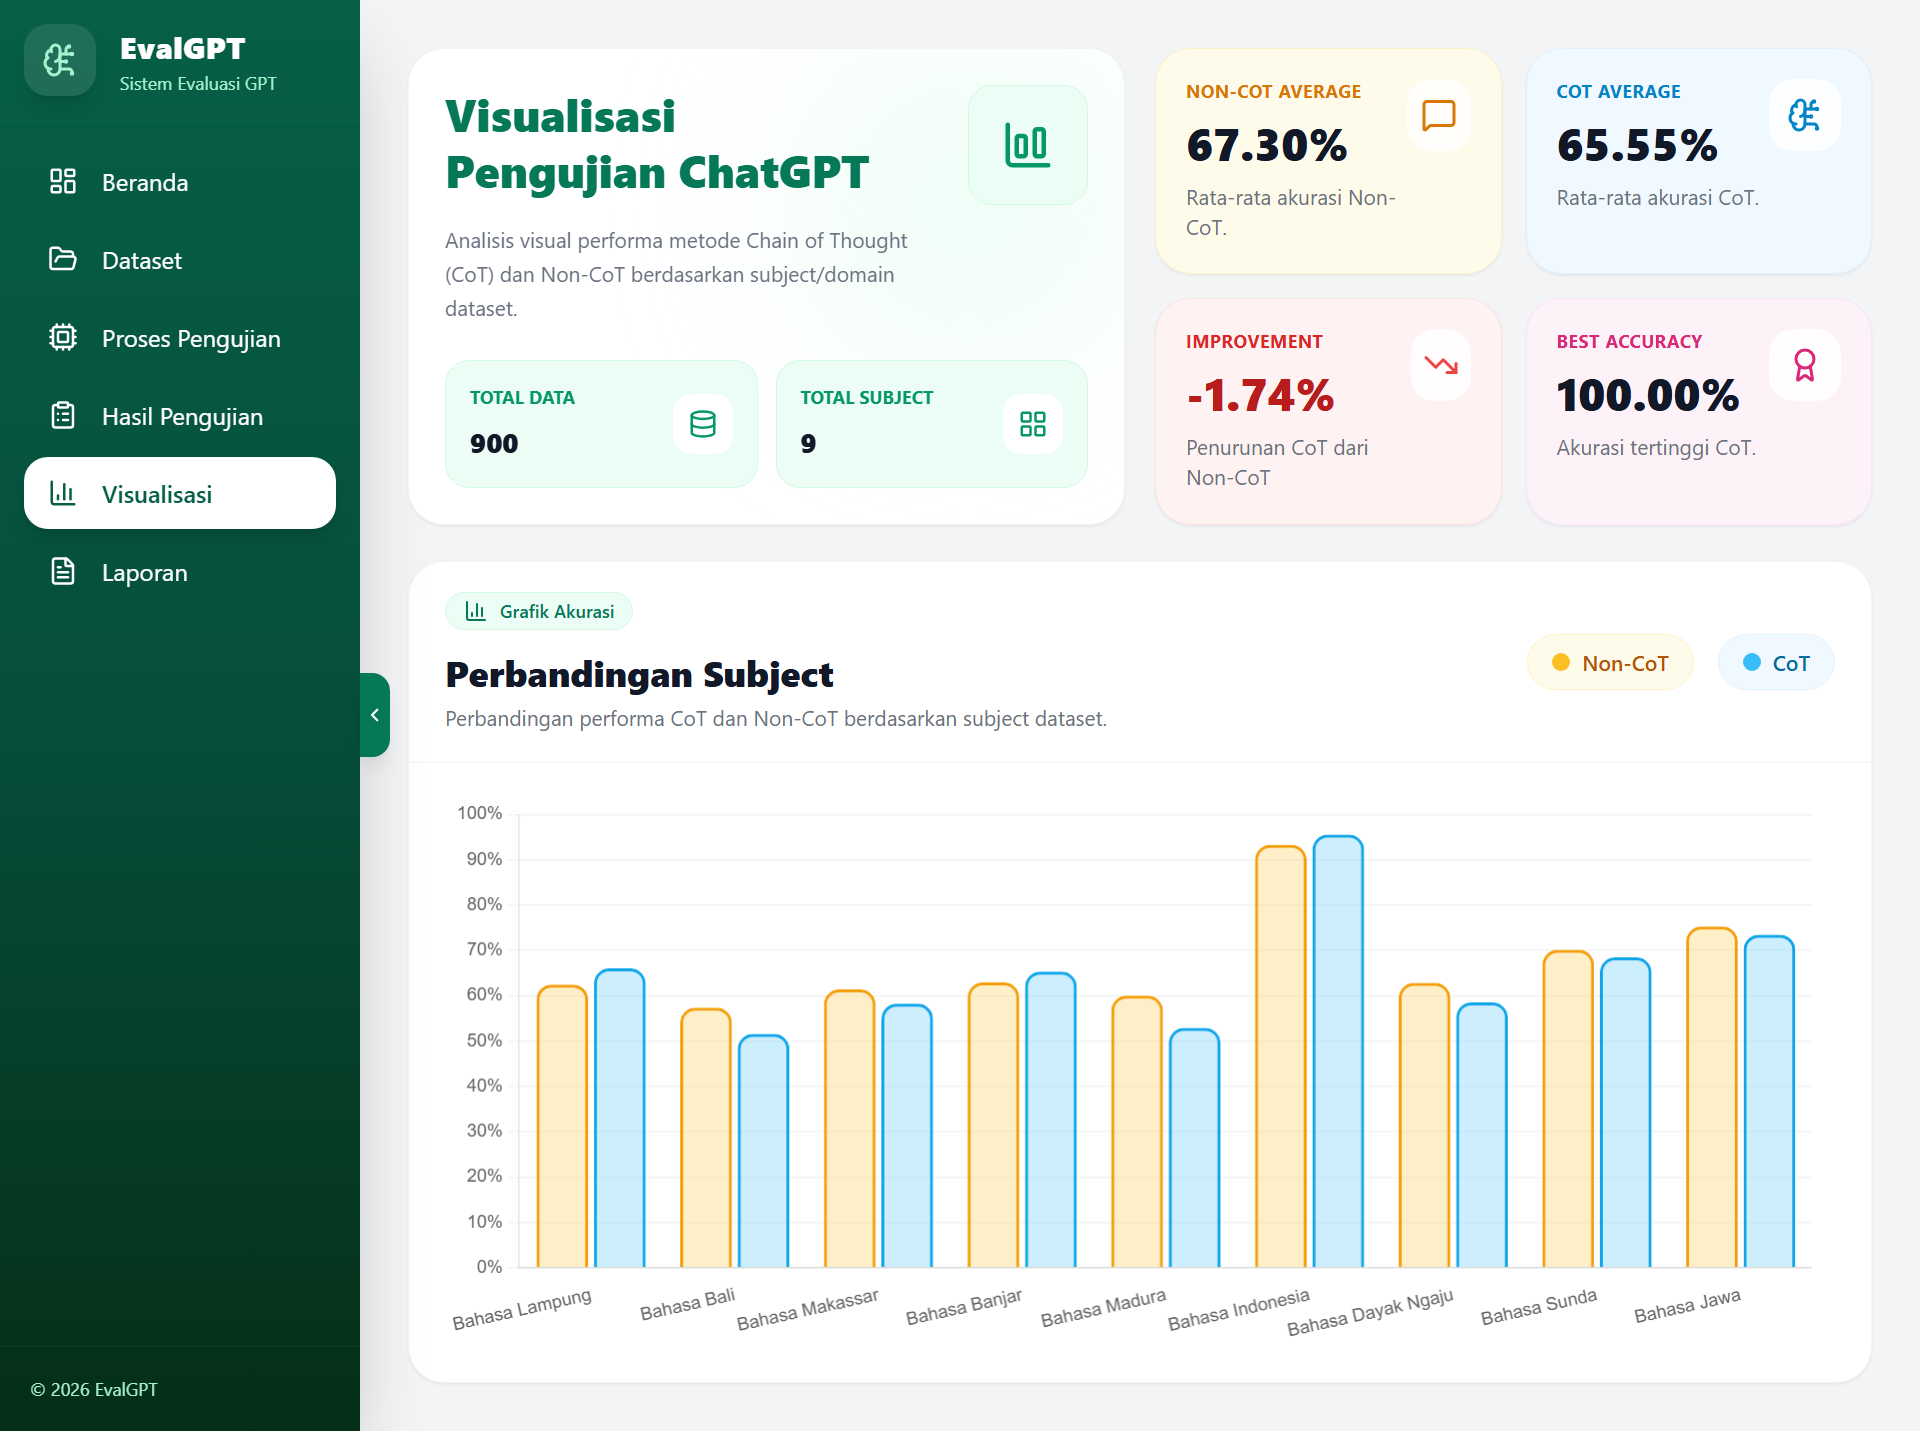
\includegraphics[width=0.72\textwidth]{skripsi_elvira_image53.png}}{\fbox{Grafik Visualisasi Hasil}}
  \caption{Visualisasi Perbandingan Skor Similarity dan Akurasi Metode CoT vs Non-CoT pada Aplikasi EvalGPT}
  \label{fig:viz_evalgpt}
\end{figure}

Tabel \ref{tab:multi_domain} dan Gambar \ref{fig:viz_evalgpt} mengungkap fakta empiris penting:
\begin{enumerate}
    \item Pada Skenario 2 dan 3, nilai \textit{similarity} Non-CoT secara konsisten lebih tinggi (68,60\% vs 68,27\% dan 70,18\% vs 69,37\%) meskipun jumlah soal benar CoT unggul tipis sebanyak 2 butir soal. Hal ini terjadi karena respons CoT sering kali menyertakan narasi elaboratif yang menambahkan jarak Levenshtein ketika format jawaban akhir tidak terisolasi sempurna.
    \item Pada \textbf{Skenario 4 (skala penuh 900 soal)}, Non-CoT berbalik unggul mutlak baik dari segi \textit{similarity} (67,30\% vs 65,55\%) maupun jumlah soal benar (469 vs 456 soal). Pada volume soal besar dengan pergantian bahasa daerah yang cepat, penalaran CoT rentan mengalami akumulasi disorientasi semantik (\textit{context drift}).
\end{enumerate}

\subsection{Analisis Trade-Off Efisiensi Komputasi (Token dan Latensi)}
Dari aspek efisiensi komputasi, metode \textit{Chain-of-Thought} membutuhkan konsumsi sumber daya yang jauh lebih masif:
\begin{itemize}
    \item \textbf{Penggunaan Token:} CoT mengonsumsi rata-rata \textbf{$5{,}18\times$ hingga $5{,}44\times$ lipat} lebih banyak token dibanding Non-CoT (misalnya pada Skenario 4: 372.965 token CoT berbanding 71.908 token Non-CoT).
    \item \textbf{Waktu Respons (Latensi):} Rata-rata waktu inferensi CoT berkisar antara \textbf{5,00--5,48 detik per soal}, atau \textbf{$3{,}5\times$ hingga $3{,}8\times$ lebih lambat} dibandingkan Non-CoT yang hanya membutuhkan \textbf{1,42--1,77 detik per soal}.
\end{itemize}
Mengingat margin peningkatan akurasi CoT yang sangat marjinal (atau bahkan menurun pada skala besar), penerapan CoT untuk tugas pemahaman bahasa daerah berbasis MCQ terbukti \textbf{tidak efisien dari segi biaya komputasi (\textit{cost-inefficient})}.

\subsection{Implementasi Antarmuka Sistem Web EvalGPT}
Sistem diimplementasikan secara terintegrasi pada aplikasi web EvalGPT. Antarmuka menyajikan modul pengunggahan dataset, konfigurasi metode inferensi (CoT/Non-CoT), eksekusi API GPT-4o mini, visualisasi metrik kemiripan berbasis Levenshtein Distance secara \textit{real-time}, serta fitur ekspor laporan ke format Excel dan PDF (Gambar \ref{fig:ui_evalgpt}).

\begin{figure}[htbp]
  \centering
  \IfFileExists{Gambar/skripsi_elvira_image49.png}{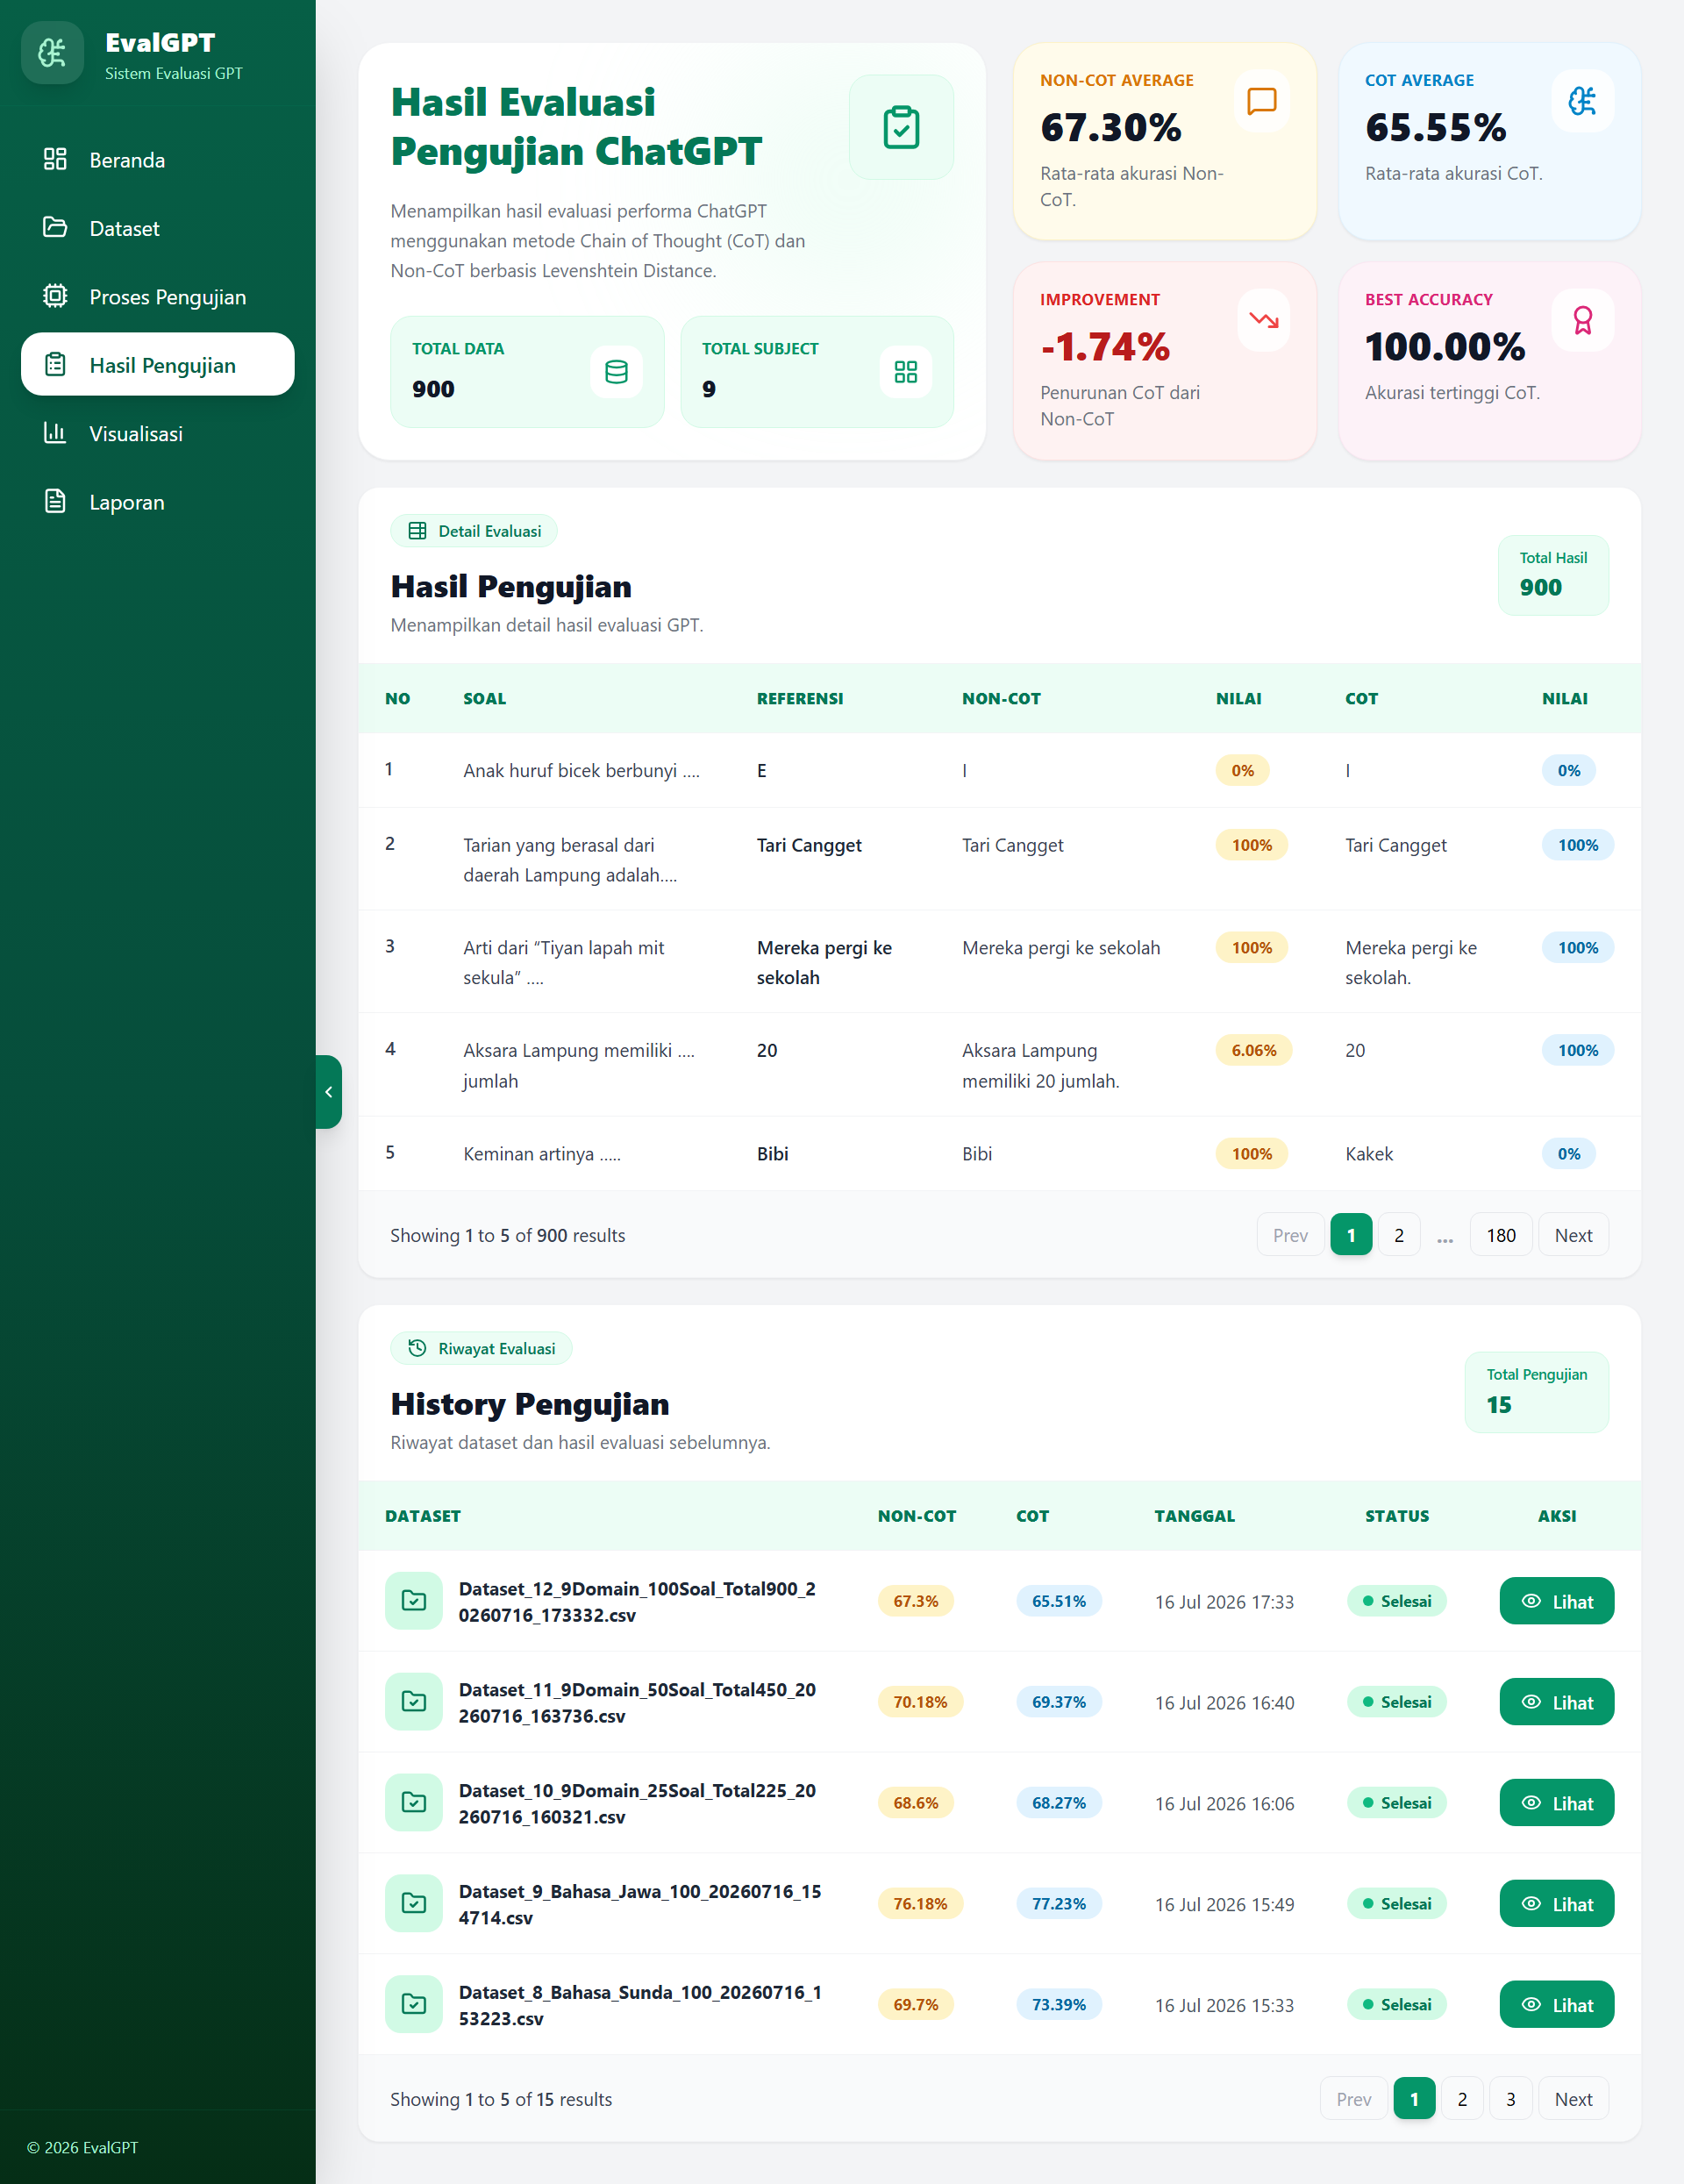
\includegraphics[width=0.72\textwidth]{skripsi_elvira_image49.png}}{\fbox{Antarmuka Hasil Pengujian EvalGPT}}
  \caption{Implementasi Antarmuka Halaman Hasil Pengujian dan Evaluasi Akurasi pada EvalGPT}
  \label{fig:ui_evalgpt}
\end{figure}

% =========================================================================
% Section 4: Conclusion
% =========================================================================
\section{KESIMPULAN DAN SARAN}

\subsection{Kesimpulan}
Berdasarkan perancangan, implementasi, dan serangkaian pengujian yang telah dilaksanakan, disimpulkan:
\begin{enumerate}
    \item Pengujian akurasi ChatGPT model GPT-4o mini pada dataset IndoMMLU domain bahasa daerah berhasil dilaksanakan menggunakan algoritma Levenshtein Distance melalui sistem otomasi EvalGPT.
    \item Metode \textit{Chain-of-Thought} (CoT) tidak memberikan peningkatan performa yang konsisten pada domain bahasa daerah. Pada pengujian per domain (Skenario 1), CoT unggul tipis dengan similarity 65,42\% (483 benar) dibanding Non-CoT 63,81\% (454 benar). Namun pada pengujian multi-domain skala besar (Skenario 4), Non-CoT justru lebih unggul dengan similarity 67,30\% (469 benar) berbanding CoT 65,55\% (456 benar).
    \item Terdapat disparitas performa linguistik yang tajam: Bahasa Indonesia mencapai akurasi tertinggi (95,92\%), diikuti Bahasa Jawa (77,23\%) dan Sunda (73,39\%), sedangkan bahasa berdaya rendah seperti Dayak Ngaju (57,88\%) dan Makassar (59,39\%) mengalami kendala pemahaman yang berat.
    \item Penerapan CoT menimbulkan penalti komputasi yang tinggi, mengonsumsi token $\approx 5{,}2$ kali lebih besar dan latensi $3{,}7$ kali lebih lama tanpa memberikan peningkatan akurasi yang sepadan.
\end{enumerate}

\subsection{Saran}
Saran untuk penelitian lanjutan meliputi:
\begin{enumerate}
    \item Mengembangkan teknik \textit{Few-Shot CoT} dengan menyertakan contoh penalaran dalam bahasa daerah lokal (\textit{in-context exemplar}) untuk memitigasi kesalahan semantik.
    \item Mengeksplorasi metode \textit{fine-tuning} model LLM sumber terbuka (\textit{open-source} seperti Llama 3 atau Mistral) menggunakan korpus leksikon bahasa daerah nusantara.
\end{enumerate}

% =========================================================================
% Acknowledgements
% =========================================================================
\section*{UCAPAN TERIMA KASIH}
Penulis menyampaikan rasa terima kasih kepada Jurusan Teknologi Informasi dan Komputer Politeknik Negeri Lhokseumawe, serta Bapak Muhammad Arhami, S.Si., M.Kom. (Pembimbing Utama) dan Bapak Muhammad Rizka, S.T., M.T. (Pembimbing Pendamping) atas segala bimbingan dan arahan akademik yang berharga.

% =========================================================================
% References (IEEE Style)
% =========================================================================
\section*{DAFTAR PUSTAKA}

\begingroup
\renewcommand{\section}[2]{}%
\begin{thebibliography}{99}
\fontsize{8pt}{10pt}\selectfont
\setlength{\itemsep}{1pt}
\setlength{\parskip}{0pt}

\bibitem{kocmi2022findings}
T. Kocmi \textit{et al.}, ``Findings of the 2022 Conference on Machine Translation (WMT22),'' in \textit{Proc. 7th Conf. Mach. Transl. (WMT)}, 2022, pp. 1--45, doi: 10.18653/v1/2022.wmt-1.1.

\bibitem{takumu2023indommlu}
Takumu, ``IndoMMLU: Indonesian Dataset for LLM Evaluation,'' \textit{AI-SCHOLAR}, 2023.

\bibitem{li2024can}
W. Li, L. Li, T. Xiang, X. Liu, W. Deng, and N. Garcia, ``Can multiple-choice questions really be useful in detecting the abilities of LLMs?,'' \textit{arXiv preprint arXiv:2403.17752}, 2024.

\bibitem{brown2020language}
T. B. Brown \textit{et al.}, ``Language Models are Few-Shot Learners,'' in \textit{Proc. Adv. Neural Inf. Process. Syst. (NeurIPS)}, 2020, pp. 1877--1901.

\bibitem{xu2024reasoning}
S. Xu \textit{et al.}, ``Reasoning before Comparison: LLM-Enhanced Semantic Similarity Metrics for Domain Specialized Text Analysis,'' \textit{arXiv preprint arXiv:2402.11398}, 2024.

\bibitem{teh2024impact}
P. L. Teh and C. F. Uwasomba, ``Impact of Large Language Models on Scholarly Publication Titles and Abstracts: A Comparative Analysis,'' \textit{J. Soc. Comput.}, vol. 5, no. 2, pp. 105--121, 2024, doi: 10.23919/JSC.2024.0011.

\bibitem{wei2023chain}
J. Wei \textit{et al.}, ``Chain-of-Thought Prompting Elicits Reasoning in Large Language Models,'' in \textit{Proc. Adv. Neural Inf. Process. Syst. (NeurIPS)}, 2022, pp. 24824--24837.

\bibitem{kojima2023large}
T. Kojima, S. S. Gu, M. Reid, Y. Matsuo, and Y. Iwasawa, ``Large Language Models are Zero-Shot Reasoners,'' in \textit{Proc. Adv. Neural Inf. Process. Syst. (NeurIPS)}, 2022, pp. 22199--22213.

\bibitem{jia2025comprehensive}
Z. Jia, S. Geng, Y. Zhao, and H. Zhang, ``Comprehensive Survey on Prompts Generating via Knowledge-Guided Chain-of-Thought,'' \textit{Int. J. Crowd Sci.}, vol. 9, no. 4, pp. 251--261, 2025, doi: 10.26599/IJCS.2024.9100038.

\bibitem{kim2023cot}
S. Kim \textit{et al.}, ``The CoT Collection: Improving Zero-shot and Few-shot Learning of Language Models via Chain-of-Thought Fine-Tuning,'' in \textit{Proc. Conf. Empir. Methods Nat. Lang. Process. (EMNLP)}, 2023, pp. 1270--1285.

\bibitem{ji2024chain}
B. Ji, H. Liu, M. Du, and S.-K. Ng, ``Chain-of-Thought Improves Text Generation with Citations in Large Language Models,'' \textit{arXiv preprint arXiv:2403.04218}, 2024.

\bibitem{lind2023comparing}
H. C. Lind-Combs, T. Bent, R. F. Holt, C. G. Clopper, and E. Brown, ``Comparing Levenshtein Distance and dynamic time warping in predicting listeners' judgments of accent distance,'' \textit{Speech Commun.}, vol. 155, p. 102987, 2023, doi: 10.1016/j.specom.2023.102987.

\bibitem{song2024sidildng}
J. Song, G. Qin, Y. Liang, J. Yan, and M. Sun, ``SIDiLDNG: A similarity-based intrusion detection system using improved Levenshtein Distance and N-gram for CAN,'' \textit{Comput. Secur.}, vol. 142, p. 103847, 2024, doi: 10.1016/j.cose.2024.103847.

\bibitem{berger2021levenshtein}
B. Berger, M. S. Waterman, and Y. W. Yu, ``Levenshtein Distance, Sequence Comparison and Biological Database Search,'' \textit{IEEE Trans. Inf. Theory}, vol. 67, no. 6, pp. 3287--3294, 2021, doi: 10.1109/TIT.2020.2996543.

\bibitem{petty2022new}
T. Petty, J. Hannig, T. I. Huszar, and H. Iyer, ``A New String Edit Distance and Applications,'' \textit{Algorithms}, vol. 15, no. 7, p. 242, 2022, doi: 10.3390/a15070242.

\bibitem{sandamette2025}
P. Sanda Mette, E. Arriyanti, S. Lailiyah, S. Widya, C. Dharma, and K. Timur, ``Penerapan Algoritma Levenshtein Distance Untuk Pengecekan Kemiripan Judul Skripsi di STMIK Widya Cipta Dharma,'' \textit{Jurnal Nasional Komputasi dan Teknologi Informasi (JNKTI)}, vol. 8, no. 3, 2025.

\bibitem{young2021levenshtein}
B. Young, T. Faris, and L. Armogida, ``Levenshtein Distance as a measure of accuracy and precision in forensic PCR-MPS methods,'' \textit{Forensic Sci. Int. Genet.}, vol. 55, p. 102594, 2021, doi: 10.1016/j.fsigen.2021.102594.

\bibitem{mugaanyi2024evaluation}
J. Mugaanyi, L. Cai, S. Cheng, C. Lu, and J. Huang, ``Evaluation of Large Language Model Performance and Reliability for Citations and References in Scholarly Writing: Cross-Disciplinary Study,'' \textit{J. Med. Internet Res.}, vol. 26, p. e52935, 2024, doi: 10.2196/52935.

\bibitem{ji2025evaluating}
K. Ji, Z. Wu, J. Han, G. Zhai, and J. Liu, ``Evaluating ChatGPT-4's performance on oral and maxillofacial queries: Chain-of-Thought and standard method,'' \textit{Front. Oral Health}, vol. 6, p. 1541976, 2025, doi: 10.3389/froh.2025.1541976.

\bibitem{suharto2025comparative}
R. N. Suharto, M. H. Z. Al Faroby, and Y. Setiawan, ``Comparative Evaluation of YOLO-based Models for Indonesian License Plate Detection and Recognition with EASY OCR,'' \textit{Procedia Comput. Sci.}, vol. 245, pp. 943--952, 2025, doi: 10.1016/j.procs.2025.09.037.

\bibitem{mohammed2025comprehensive}
A. Mohammed and R. Kora, ``A Comprehensive Overview and Analysis of Large Language Models: Trends and Challenges,'' \textit{IEEE Access}, vol. 13, pp. 24501--24520, 2025, doi: 10.1109/ACCESS.2025.3573955.

\bibitem{hakansson2024generative}
A. H\aa kansson and G. Phillips-Wren, ``Generative AI and Large Language Models -- Benefits, Drawbacks, Future and Recommendations,'' \textit{Procedia Comput. Sci.}, vol. 240, pp. 5458--5468, 2024, doi: 10.1016/j.procs.2024.09.689.

\bibitem{openai2024gpt4omini}
OpenAI, ``GPT-4o mini: Advancing Cost-Efficient Intelligence,'' \textit{OpenAI Blog}, 2024. [Daring]. Tersedia: \url{https://openai.com/index/gpt-4o-mini-advancing-cost-efficient-intelligence/}.

\bibitem{favero2025advancing}
N. Favero, F. Salute, and D. Hardt, ``Advancing Academic Chatbots: Evaluation of Non Traditional Outputs,'' \textit{arXiv preprint arXiv:2512.00991}, 2025.

\bibitem{reynolds2021prompt}
L. Reynolds and K. McDonell, ``Prompt Programming for Large Language Models: Beyond the Few-Shot Paradigm,'' in \textit{Proc. CHI Conf. Hum. Factors Comput. Syst. (CHI)}, 2021, pp. 1--7, doi: 10.1145/3411764.3445768.

\end{thebibliography}
\endgroup

\end{document}
